% -----------------------------------------------
% Template for ICMC SMC 2014
% adapted and corrected from the template for SMC 2013,  which was adapted from that of  SMC 2012, which was adapted from that of SMC 2011
% -----------------------------------------------

\documentclass{article}
\usepackage{icmcsmc2014}
\usepackage[]{biblatex}
\addbibresource{SpatDIF.bib}
\usepackage{times}
\usepackage{ifpdf}
\usepackage[english]{babel}
\usepackage{listings}
\usepackage{enumitem}
\sloppy
\setlist[itemize]{itemsep=0.0pt, topsep=1.5pt}

%\usepackage{cite}

%%%%%%%%%%%%%%%%%%%%%%%% Some useful packages %%%%%%%%%%%%%%%%%%%%%%%%%%%%%%%
%%%%%%%%%%%%%%%%%%%%%%%% See related documentation %%%%%%%%%%%%%%%%%%%%%%%%%%
%\usepackage{amsmath} % popular packages from Am. Math. Soc. Please use the 
%\usepackage{amssymb} % related math environments (split, subequation, cases,
%\usepackage{amsfonts}% multline, etc.)
%\usepackage{bm}      % Bold Math package, defines the command \bf{}
%\usepackage{paralist}% extended list environments
%%subfig.sty is the modern replacement for subfigure.sty. However, subfig.sty 
%%requires and automatically loads caption.sty which overrides class handling 
%%of captions. To prevent this problem, preload caption.sty with caption=false 
%\usepackage[caption=false]{caption}
%\usepackage[font=footnotesize]{subfig}


%user defined variables
\def\papertitle{The SpatDIF library - Concepts and Practical Applications in Audio Software}
\def\firstauthor{Jan C. Schacher}
\def\secondauthor{Chikashi Miyama}
\def\thirdauthor{Trond Lossius}

% adds the automatic
% Saves a lot of ouptut space in PDF... after conversion with the distiller
% Delete if you cannot get PS fonts working on your system.

% pdf-tex settings: detect automatically if run by latex or pdflatex
\newif\ifpdf
\ifx\pdfoutput\relax
\else
   \ifcase\pdfoutput
      \pdffalse
   \else
      \pdftrue
\fi

% \ifpdf % compiling with pdflatex
  \usepackage[pdftex,
    pdftitle={\papertitle},
    pdfauthor={\firstauthor, \secondauthor, \thirdauthor},
    bookmarksnumbered, % use section numbers with bookmarks
    pdfstartview=XYZ % start with zoom=100% instead of full screen; 
                     % especially useful if working with a big screen :-)
   ]{hyperref}
  %\pdfcompresslevel=9

  \usepackage[pdftex]{graphicx}
  % declare the path(s) where your graphic files are and their extensions so 
  %you won't have to specify these with every instance of \includegraphics
  % \graphicspath{./figures/}
  \DeclareGraphicsExtensions{.pdf,.jpeg,.png}

  \usepackage[figure,table]{hypcap}
	
% \else % compiling with latex
%   \usepackage[dvips,
%     bookmarksnumbered, % use section numbers with bookmarks
%     pdfstartview=XYZ % start with zoom=100% instead of full screen
%   ]{hyperref}  % hyperrefs are active in the pdf file after conversion
% 
%   \usepackage[dvips]{epsfig,graphicx}
%   % declare the path(s) where your graphic files are and their extensions so 
%   %you won't have to specify these with every instance of \includegraphics
%   \graphicspath{./figures/}
%   % \DeclareGraphicsExtensions{.eps}
% 
%   \usepackage[figure,table]{hypcap}
% \fi

%setup the hyperref package - make the links black without a surrounding frame
\hypersetup{
    colorlinks,%
    citecolor=black,%
    filecolor=black,%
    linkcolor=black,%
    urlcolor=black
}


% Title.
% ------
\title{\papertitle}

% Authors
% Please note that submissions are NOT anonymous, therefore 
% authors' names have to be VISIBLE in your manuscript. 
%
% Single address
% To use with only one author or several with the same address
% ---------------
%\oneauthor
%   {\firstauthor} {Affiliation1 \\ %
%     {\tt \href{mailto:author1@smcnetwork.org}{author1@smcnetwork.org}}}

%Two addresses
%--------------
% \twoauthors
%   {\firstauthor} {Affiliation1 \\ %
%     {\tt \href{mailto:author1@smcnetwork.org}{author1@smcnetwork.org}}}
%   {\secondauthor} {Affiliation2 \\ %
%     {\tt \href{mailto:author2@smcnetwork.org}{author2@smcnetwork.org}}}

% Three addresses
% --------------
 \threeauthors
   {\firstauthor} {Zurich University of the Arts\\
   Institute for Computer Music\\ and Sound Technology ICST\\
     {\tt \href{jan.schacher@zhdk.ch}{jan.schacher@zhdk.ch}}}
   {\secondauthor} {University of Music, Cologne\\ 
   Studio for Electronic Music\\
     {\tt \href{me@chikashi.net}{me@chikashi.net}}}
   {\thirdauthor} { Bergen Center for Electronic Arts BEK\\ %
     {\tt \href{trond.lossius@bek.no}{trond.lossius@bek.no} }
}


% ***************************************** the document starts here ***************

\begin{document}
%
\capstartfalse
\maketitle
\capstarttrue
%
\begin{abstract}
The development and specification of SpatDIF, the Spatial Sound Description Interchange Format, is complemented with actual implementations in software in order to become available in various audio software environments.
This article discusses the current state of the development of a software library called `libspatdif', whose purpose is to provide a reference implementation of SpatDIF and demonstrate its best-use practices.
In addition, the design principles derived from the concepts and specifications of SpatDIF, the class structure of the software library, and the concrete implementations demonstrating its usage in computer music applications is presented.
\end{abstract}

\section{Background}
SpatDIF, the Spatial Sound Description Interchange Format, presents a structured syntax for describing spatial audio information, addressing the different tasks involved in creating and performing spatial sound scenes.
The goal of the SpatDIF approach is to simplify and enhance the methods of creating spatial sound content and to enable the exchange of between otherwise incompatible software. 
SpatDIF proposes a simple and extensible format as well as best-practice examples for storing and transmitting spatial sound scene descriptions. 
It encourages portability and the exchange of compositions between venues with different surround audio infrastructures. 
SpatDIF also fosters collaboration between artists such as composers, musicians, sound installation artists, and sound designers, as well as researchers in the fields of acoustics, musicology, sound engineering and virtual reality.
SpatDIF is developed in a collaborative effort and has evolved over a number of years. 
The community and all related information can be found at \url{www.spatdif.org}.%\footnotesize{\url{www.spatdif.org}}.\normalsize

SpatDIF was coined in \citeyear{peters_caa07} \cite{peters_caa07} when Peters posited the need for a format describing spatial sound scenes in a structured way, since at that time all of the available spatial rendering systems used self-contained, proprietary syntax- and data-formats.
Through a panel discussion \cite{2008ICMCpanel, Peters:2008spatdif} and other meetings and workshops, the scope and concepts of SpatDIF were extended, refined, and consolidated.
After an extended process the SpatDIF specification was informally presented to the spatial sound community at the ICMC in Huddersfield in August 2011 and at a workshop at the TU-Berlin in September 2011.
The responses in these meetings suggested the urgent need for a lightweight and easy to implement spatial sound scene standard, which would contrast the complex MPEG-4 scene description specification \cite{scheirer1999audiobifs}.

The completion of a first usable version of the specifications \cite{SpatDIF_03} defining the core descriptors and a few indispensable additional descriptors was achieved the following year. The publication of this project milestone at the SMC in Copenhagen \cite{SpatDIF_SMC12} won a best paper award and was subsequently published in the Computer Music Journal \cite{Peters:2013SpatDifCMJ}.
This encouragement incited the group to tackle the task of proving that the concept would work in actual software.

A central principle for SpatDIF is the conceptual separation of authoring and rendering of spatial sound scenes or pieces. They may occur at separate times using the same or differing infrastructure, at separate places either simultaneously or with a long time between the two and of course through a mixture of these factors. 
The exact modality should not have to be determined at the outset.

In addition to the separation of the basic functionalities two principal use-cases can be distinguished.
The first scenario is focused on storing spatial audio pieces on a support for future playback. 
The second scenario deals with streamed content and scene information in real- or near real-time.
For these applications SpatDIF formulates a concise semantic structure that is capable of carrying all the information relevant for preserving a sound scene, without being tied to a specific implementation or technical method.
Since SpatDIF is a syntax rather than a programming interface or file-format it may be represented in any of the current or future structured mark-up languages or messaging systems.
It describes only those aspects required for the storage and transmission of \emph{spatial sound information}.
Because a complete work typically contains aspects that are outside the realm of spatial sound scenes, SpatDIF provides descriptors to link these aspects to the spatial dimensions, but only to the extent necessary.
% For example, the description of media-streams in SpatDIF is necessary in order to define the storage location or origin of the audio present in the scene.
% For example, to be able to render the audio objects with the correct audio content in the spatial scene, the storage location of the audio content needs to be defined via SpatDIF's media resources.
For example, the description of media-streams in the Media extension is necessary in order to describe from where the sounding content of the scene originates.

\section{libspatdif Concepts}\label{sec:libspatdif_concepts}

In this article we present the development and implementation of a software tool is aimed at an easy integration of SpatDIF into existing software.
The concepts and guidelines0.95 laid down in the SpatDIF specifications are implemented in a software-library.
In addition to the low-level library to demonstrate the usage of SpatDIF, example applications which utilise this library were created and will be discussed below.
The use of this library is demonstrated in externals for MaxMSP and PureData and in an application written entirely in C++ in the creative coding environment openFrameworks \footnote{\url{http://www.openframeworks.cc}\\all URIs accessed 1. April 2014 }.

After establishing a coherent specification with example use cases in textual form only, the next development step is the implementation of software that embodies the specified concepts.
For this purpose a platform-independent software library was designed and is now implemented.
By providing a software library rather than just a complete software application, implementations in many different software environments are facilitated, which is one of the goals of the project.
The library is in charge of holding one or more spatial audio scenes and provide ways to read and write elements to and from this scenes, either directly from native code or via OSC-formatted messages, that may originate from within the application or or come in from an external source via the network. 

\subsection{Library Class Structure}\label{sec:class_structure}

\begin{figure}[h]
% \centerline{ 
	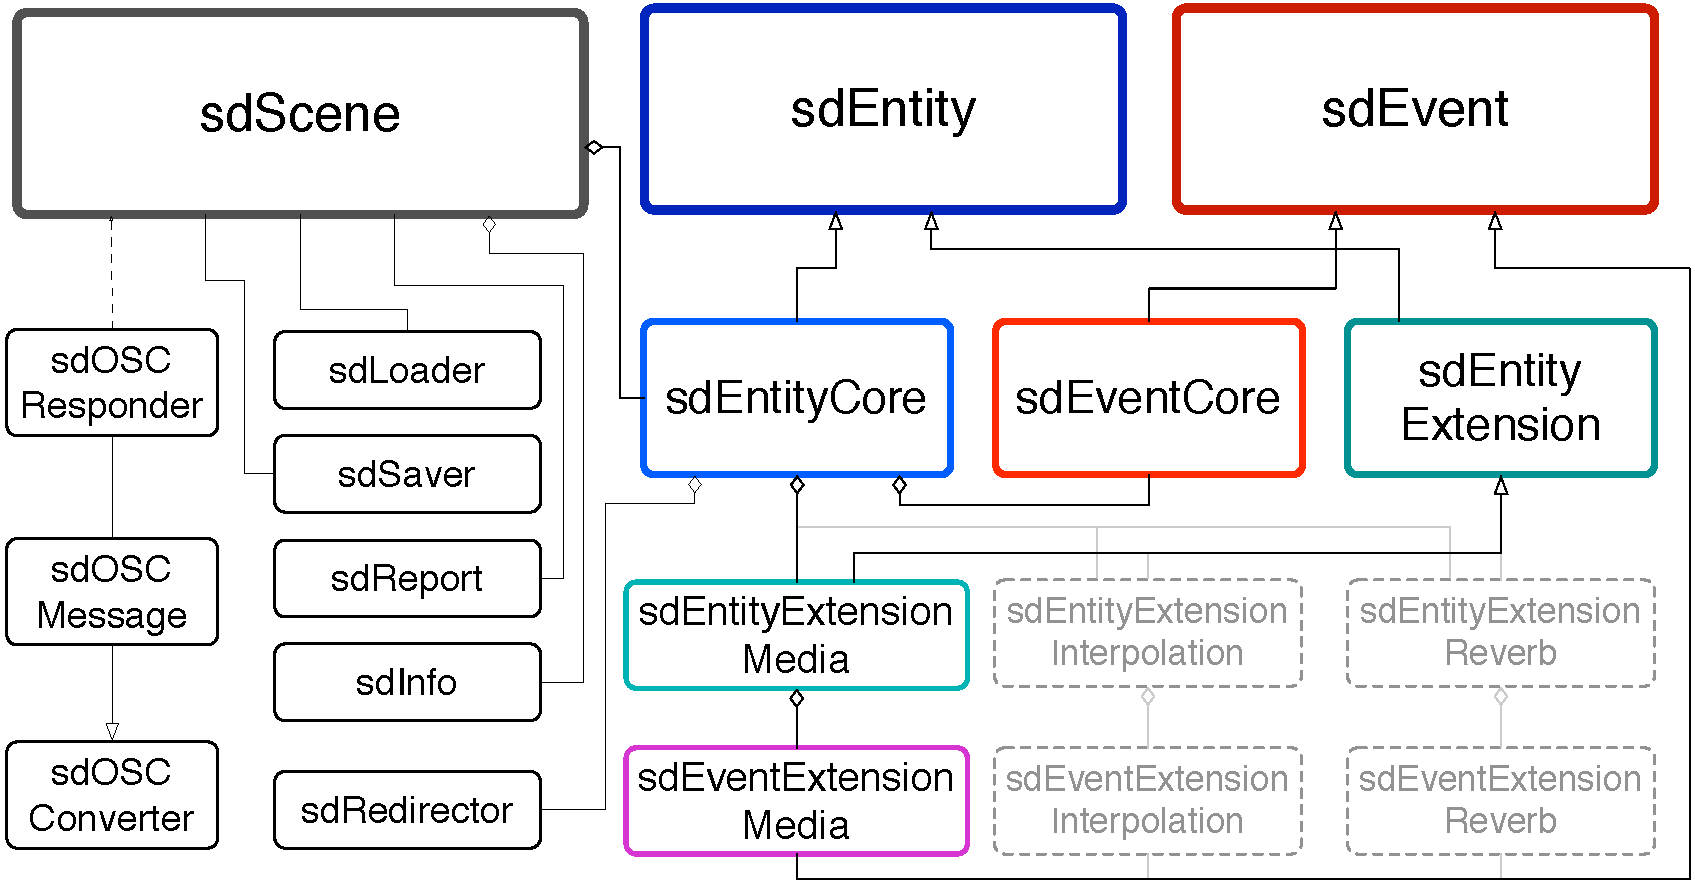
\includegraphics[width=0.98\columnwidth]{class_diagram.pdf}
% }
	\caption{Simplified class hierarchy of the SpatDIF software library.
\label{fig:class_structure}
}
\end{figure}

The class hierarchy described here is intended to show the relationship between the scene and its contents, as well as their hierarchical dependencies (see Figure \ref{fig:class_structure}). 
An instance of \emph{sdScene} class represents a SpatDIF scene and maintains instances of \emph{sdEntityCore}. The functionalities of \emph{sdEntityCore} may be extended by the descendants of \emph{sdEntityExtension}. 
The activation and deactivation of the extension are global within a scene, therefore \emph{sdScene} is also responsible for the extension handling.
Each instance of \emph{sdEntityCore} maintains instances of \emph{sdEvent}, which represent events of the entity they are attached to.

The following are brief descriptions of the most important classes.

\begin{itemize}[leftmargin=-0.0mm]
\item[] \emph{sdScene}\\
An instance of \emph{sdScene} maintains all data associated to a SpatDIF scene. This class offers clients the following three main functionalities: Addition, deletion and modification of \textbf{entities} in the scene; Addition and modification of the \textbf{meta data} associated to the scene; Activation and deactivation of the \textbf{extensions} in the scene.

Once the client activates an extension in a scene, \emph{sdScene} automatically adds extended functionalities and allocates extra buffers to all existing and newly created instances of \emph{sdEntityCore}. 
Symmetrically, when deactivating an extension, \emph{sdScene} removes all extended functionalities and previously allocated buffers from all existing \emph{sdEntitieCores}, leading to the deletion of all data stored in the extension buffers.

\item[] \emph{sdEvent}\\
This is a pure abstract class of event, that maintains the following three data items: \textbf{time} - absolute time of the event; \textbf{descriptor} - type of event; \textbf{value} - actual data.

\item[] \emph{sdEntity}\\
This is a pure abstract class of entity in SpatDIF scenes. Basic functionalities, such as addition, deletion, and modification of events are implemented.

\item[] \emph{sdEntityCore}\\
An instance of \emph{sdEntityCore} maintains events with SpatDIF core descriptors and a vector storing instances of SpatDIF extensions. 
This class replies to queries from the client about events, e.g. if a client asks a \emph{sdEntityCore} a value of a certain descriptor at a specific time, the \emph{sdEntityCore} returns the value. 
The client is able to raise an query about multiple events within a certain time frame and filter events by descriptors. 

\item[] \emph{sdEntityExtension}\\
This is a pure abstract class of extensions. The descendants of this class. e.g. \emph{sdEntityExtensionMedia} handles the events with extended descriptors. 
If a client activates an extension in a scene, each existing instance of \emph{sdEntityCore} instantiates the designated subclass of \emph{sdEntityExtension} and register it in its internal vector.

\item[] \emph{sdLoader/sdSaver}\\
These two classes provide several utility functions and enable clients to create an instance of \emph{sdScene} from a XML, JSON, or YAML string and vice versa. 
In order to maintain platform independence and to achieve maximum flexibility, the library does not handle files directly, the client software is responsible for the file management. 
These functions use two external libraries for parsing of markup formatted strings: TinyXML-2\footnote{\url{http://www.grinninglizard.com/tinyxml} } and libjson\footnote{\url{http://sourceforge.net/projects/libjson} }.
\end{itemize}

% TODO @Trond/Chikashi decide if the code-examples should stay in this paper, since this paper is mainly about the externals an should be different enough from the JSSA paper from last december. Perhaps an extract from the turena's file would be more appropriate here? [jasch]
\subsection{Simple Code Example}
The following code listing shows how to load an XML-formatted string obtained from a SpatDIF file into an \emph{sdScene} and query the entity called `insect' for the first occurrence of an event which contains a position and a media descriptor.

\lstinputlisting[columns=fullflexible, breaklines=true, numbers=left,xleftmargin=3.0em,frame=none,framexleftmargin=0.0em, basicstyle=\scriptsize\ttfamily]{example_code2.cpp} 

\noindent The code produces this console-output: 
\lstinputlisting[columns=fullflexible,breaklines=true,numbers=none,xleftmargin=1.0em, basicstyle=\scriptsize\ttfamily]{code_output.txt} 

\noindent 
The following processes are executed in the example:

\noindent Line 1: the \emph{sdLoader::sceneFromXML} function loads a scene from an XML formatted string.

\noindent Line 2: A pointer to an entity named `insect' is obtained by the \emph{scene.getEntity} function.

\noindent Lines 3 -- 4: Entity `insect' is requested for the first event with position and media location descriptor.

\noindent Line 5: Query `insect' entity for its name.

\noindent Lines 6 -- 8: Post values and time of events.

\section{Introducing the SpatDIF External}
Even though the SpatDIF syntax is an implementation-independent specification, rather than a concrete software interface, the actual value of using it only becomes evident in concrete applications. And even if SpatDIF was developed with a number of different usage scenarios in mind, the ones most closely associated with these authors' practices are electro-acoustic surround audio compositions for concerts or installations or real-time spatialisation in computer music performance.
Therefore the primary application for the SpatDIF library lies in an implementation in real-time capable audio software.

\subsection{Concepts and Practical Usage}\label{subsec:concepts}
In order to explore the methods and actual handling of the libspatdif in a real situation, a dual testbed was implemented as externals for MaxMSP and Pure Data. 
In addition an example application with a limited feature-set was tested in openFrameworks, mainly to establish and test a workflow done entirely in the C++ language.

There are a number of concepts that need to be taken into account when using the library.
These inform the design of the implementations shown here.

The library serves as a data-storage for audio scenes that needs to be queried for its information in specific ways.
It doesn't provide a scheduling mechanism of its own, rather, the client application is responsible for executing all time-related functions.
This design choice is explicitly geared towards temporal flexibility, i.e. slowing down or speeding up playback, jumping an cueing, which are features that can only properly be implemented by the end-user.

There are two main interfaces for the library, the native call and the OSC-command.
The native commands call functions of the library within C/C++ code whereas the OSC-commands get handed to the library as messages conforming to the OSC syntax.
The library doesn't implement network socket handling functionalities, this is the client environment's task.
In order to input and output information directly to/from the scene, the name-space is described with hierarchical addresses that have to conform to the SpatDIF specification.
In the implementation of the externals, the input of elements into the scene stays in the OSC-style with a slash delimited format, whereas in the output from the scene the addresses are converted to a space-delimited format to avoid a dependency on an additional OSC-parser.

Additional commands that are directly addressing functions of the library have a different syntax, which is not part of the SpatDIF specifications, but rather specific to the implementation of the library.
These \emph{/spatdifcmd} messages concern the querying of information from the library and the setting and getting of variables necessary for the executing the queries.

File operations are not functions of the library proper.
It is the externals in MaxMSP and PureData that implement the required file loading and saving methods, which are specific to their own environment. 
 % TODO: maybe a switch could be implemented to change this behavior back and forth?


\subsection{Playback}\label{sec:Playback}

\begin{figure}[httb]
	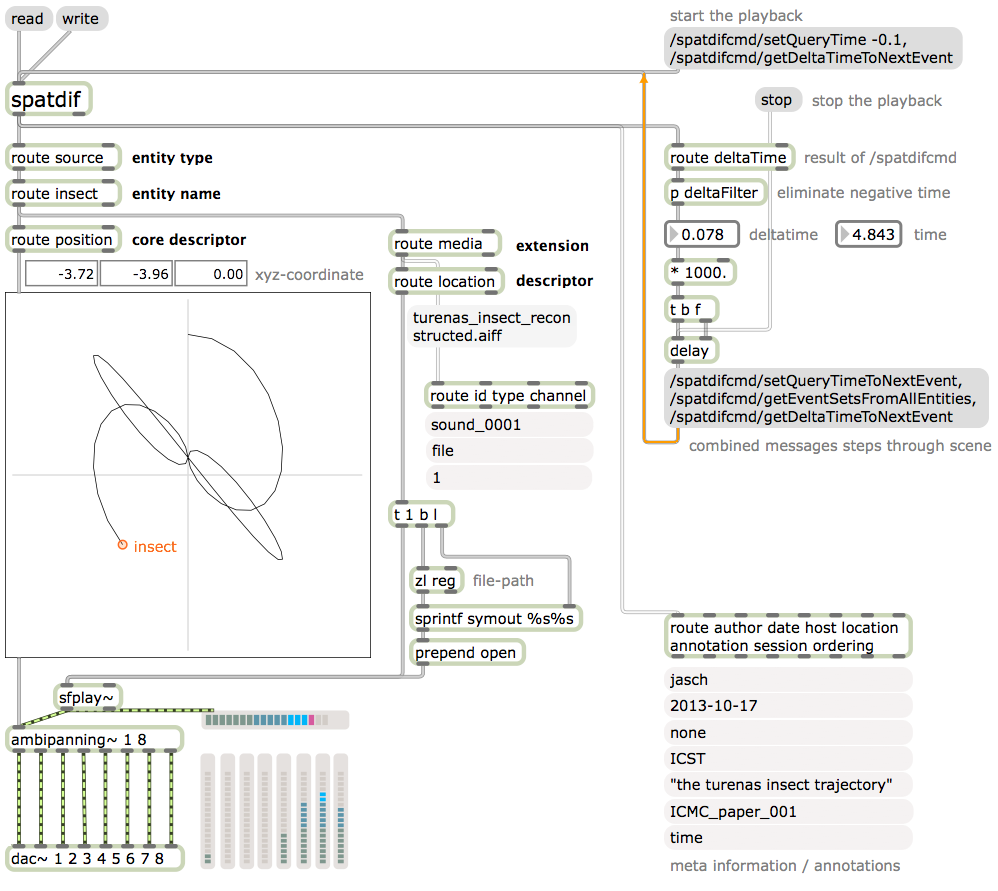
\includegraphics[width=0.98\columnwidth]{recording_maxpatch.png}
	\caption{Max external implementation of spatDIF, playing the Lissajous trajectory from Chowning's `Turenas'.} 
	\label{fig:screenshot}
\end{figure}

The first example shown here centres around SpatDIF file-handling and playback of a scene in a multichannel setup.
Figure \ref{fig:screenshot} shows a simplified monophonic setup in MaxMSP.
This workflow makes a few assumptions which are not limitations of libspatdif as such, but help to clarify the concepts.
The program demonstrates the rendering of an existing scene, which is in this instance the `insect' trajectory from John Chowning's ``Turenas'' (1972) \cite{chowningturenas}.
The scene is stored on disk in a SpatDIF-formatted XML-file together with the audio content as sound-file.
After reading the scene from disk, the meta section can be parsed to obtain annotation information, as shown in the lower right.

In a fully dynamic system, additional information is required to set up the rendering algorithm.
For this purpose queries are made to the library to obtain information about the number of entities present in the scene and the names of the entities as well as the extensions that are present.\footnote{For more specific information about the concept of extensions in SpatDIF, please refer to \cite{SpatDIF_SMC12, Peters:2013SpatDifCMJ, SpatDIF_03}. }
This allows determine the number of playback voices and to set up the hierarchical message routing according to the names of entities.
In this example this step is omitted and only one playback voice is implemented with a hard-coded message routing set to the entity-type of \emph{source} and the entity-name called \emph{insect}.
Subsequently, the messages are routed to obtain the \emph{position} core-descriptor required for the spatialisation process as well as the \emph{media} extension with the \emph{location} descriptor necessary to load files for playback.
The sound-file player, visualisation and spatialisation algorithms \cite{schacher7Years} shown here represent the minimal case and should of course be more fully implemented.

As mentioned earlier the library does not have its own scheduling mechanism. 
In this example this becomes apparent and therefore it demonstrates the method for time-based playback.
In the right half of the example are shown the \emph{spatdifmds} necessary to run iteratively run through the scene.
The basic action is to Ask with \emph{getDeltaTimeToNextEvent} for the delta times between subsequent events.
The command \emph{setQueryTimeToNextEvent} sets the query time variable to the next event, then the library gets queried for all the events at that point in time with \emph{getEventSetsFromAllEntities}, and finally the time to wait until the next event is queried again.
These commands form a loop that steps through the scene.
The timing is executed by a delay which waits the appropriate amount of time to the next event before re-triggering the same sequence.


















\subsection{Recording}\label{sub:body}
example text

\section{Future work}
example text


\begin{acknowledgments}
example text
\end{acknowledgments} 

%%%%%%%%%%%%%%%%%%%%%%%%%%%%%%%%%%%%%%%%%%%%%%%%%%%%%%%%%%%%%%%%%%%%%%%%%%%%%
%bibliography here
% \bibliography{SpatDIF.bib}
\printbibliography

\end{document}
